\chapter{A Method For Video Face Clustering Method}
\label{chap:video_face_clustering}

This chapter describes the core of this dissertation, which is a method for \emph{Video Face Clustering}.
It consists of detecting and grouping faces from different video frames~(ideally from the same actors) extracted from a video file.
Figure \ref{fig:video_face_clustering} depicts this process, and each of its steps is described in the next paragraphs.

\begin{figure*}[!ht]
    \centering
    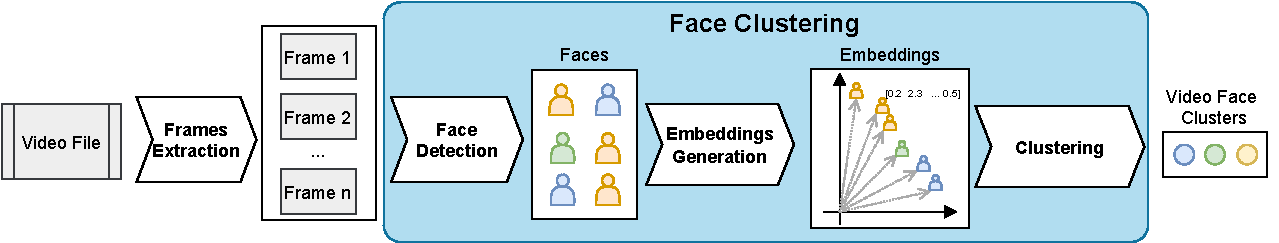
\includegraphics[width=\textwidth]{img/face_clustering/video_face_clustering.pdf}
    \caption{Video face clustering process.}
    \label{fig:video_face_clustering}
\end{figure*}


First, we perform \textit{Frames Extraction} by receiving a video file as input and extracting its frames according to a given frame rate. 
These frames are used as a set of images for the next step.

The \textit{Face Detection} step uses an object detection model for detecting faces in each of its images.
In general, any object detection model can identify which, among a known set of objects, are present in the image, and provides information about their positions.
In our case, objects are faces and, therefore, the face detection model is responsible for returning the bounding boxes of the faces present in the image, specified by the $x$ and $y$ axes coordinates of the upper-left corner and of the lower-right corner of the rectangle that establishes the visual limits that encapsulate each face. 
With these bounding boxes, we can isolate and extract the bounded images, obtaining a dataset composed of images of faces only.


The objective of the \textit{Embeddings Generation} step is to represent each face image as a vector in $\mathbb{R}^{n}$.
To achieve that, it processes each of the faces generated in the previous step through a CNN, generating embeddings. 
An embedding is a representation of the input in a lower-dimensional space.
Ideally, an embedding captures some semantics of the input, e.g. by placing semantically similar inputs close together in the embedding space.
At the end of this step, we have all faces represented as embeddings.

In the \textit{Clustering} step, we group embeddings and, consequently, faces that are close in the embedding space using a clustering algorithm. 
Clustering is the task of dividing a set of data points, embeddings in this case, into groups~(clusters) such that data points in a given group are similar to other data points in the same group and dissimilar to the data points in other groups.
The clustering process should produce a partition of the dataset, i.e., each generated cluster represents a specific person, and the union of all clusters covers the whole dataset. 
It is common for clustering algorithms to require the number of clusters in advance.
However, in the context of \emph{Video Face Clustering}, we do not know this number in advance, that is the number of actors in the video. 
For that reason, we have designed a strategy for automatically choosing an adequate number of clusters.
Section \ref{subsec:unknown_nclusters} describes this strategy.

\section{Iterative Strategy for Unknown Number of Clusters}
\label{subsec:unknown_nclusters}

In this Section, we define a strategy based on the \emph{Silhouette Score} ($s$) \cite{rousseeuw1987silhouettes} to choose an adequate clustering configuration.
The \emph{Silhouette Score}~\cite{rousseeuw1987silhouettes} corresponds to the mean of the \emph{Silhouette Coefficient} of all samples.
This coefficient ($S$) for each sample is 

\begin{equation}
\label{equation:Silh}
    S = \frac{b-a}{max(a,b)} 
\vspace{1em}
\end{equation}
%%
where $a$ is the mean distance from a sample to all other samples in the same cluster, and $b$ is the mean distance from a sample to all other samples in the closest cluster to that sample.
In this way, the best value is 1 and the worst is -1. Values close to 0 indicate overlapping clusters, whereas negative values usually indicate that a sample has been assigned to the wrong cluster since a different cluster is more similar.

With this strategy~(see Algorithm 1), we increase the number of clusters until the maximum \emph{Silhouette Score} decreases no more than $t$ times in a row or until it reaches the maximum number of clusters~(lines 5-18), which is the number of embeddings~($|e|$).
The \texttt{Clustering} procedure (line 7)
can be substituted by any clustering algorithm that requires the number of clusters in advance.
When the iteration stops, we return the clustering configuration with the highest \emph{Silhouette Score}.
Since this score requires at least two clusters, it would not be possible to compute it for a clustering configuration with only one cluster~(there are only faces of a single actor).
To overcome this problem, we start with 2 clusters consecutively increasing it as described above. Then, if the returned clustering configuration has a \emph{Silhouette Score} smaller than a threshold $\omega$, that probably indicates overlapping, we say that all faces belong to one single cluster~(lines 19-20). 

\begin{algorithm}
\small
\caption{Iteratively finding the best clustering configuration for unknown number of clusters.}\label{clustering_alg}
\begin{algorithmic}[1]
\Procedure{BlindClustering}{$e, t,\omega$}\
\State $n_K\gets 1$
\State $s_{max}\gets -1$
\State $t_{cur}\gets 0$ 

\While{$t_{cur} \leq t \And n_K < |e|$}
    \State $n_K\gets n_K+1$
    \State $K_{cur}\gets Clustering(e, n_K)$
    \State $s \gets SilhouetteScore(K_{cur})$
    \If{$s < s_{max}$}
        \State $t_{cur}\gets t_{cur}+1$
    \Else
        \State $K\gets K_{cur}$
        \State $t_{cur}\gets 0$
        
        \If{$s > s_{max}$}
            \State $s_{max} \gets s$
        \EndIf
    \EndIf
\EndWhile
\If{$s_{max} < \omega$}
    \State $K\gets OneCluster(e)$
\EndIf
\State \textbf{return} $K$
\EndProcedure
\end{algorithmic}
\end{algorithm}


By the end of this process, we expect to have the spatiotemporal localization of the actors present in a video file.
Figure \ref{fig:timeline} shows an example of the results achieved by our \emph{Video Face Clustering} method. It contains a timeline of a video with lines coloring the segments that each actor appears in.

\begin{figure}[!ht]
    \centering
    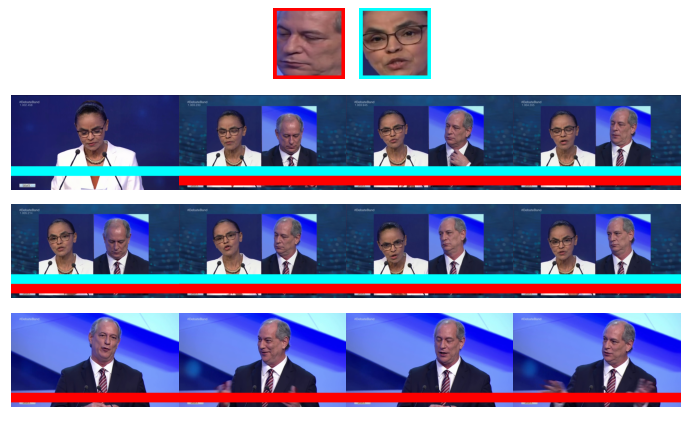
\includegraphics[width=0.65\linewidth]{img/face_clustering/example_localization.png}
    \caption{Example of spatiotemporal localization.}
    \label{fig:timeline}
\end{figure}

The following three chapters describe the applications we investigate in this dissertation. 
These three applications propose novel approaches for tasks in video using spatiotemporal localization of actors through \emph{Video Face Clustering}.

